\chapter{Evaluation and Analysis}

In the first part of this section we briefly depict the nature of the data set used for evaluation of the models and discuss some specifics of the implementation. In the next part we present the results of our analysis.

\section{Data Set}

For the analysis we used data from the online system for practicing geography\footnote{\url{http://www.slepemapy.cz}}~\cite{Papousek2014}. The data set contains more than 10~million answers from thousands of unique users~\cite{Papousek2015}. The data were filtered to contain only students with at least 50 answers and usually divided into 5 data sets, each containing at least 30 thousand answers. The answers of students who registered before the oldest question in the data set was answered were removed since it could temper with the results (considering we are interested primarily in models based on timing information).

\section{Toolchain}

The models were implemented in Python programming language. Experiments were performed in the Jupyter Notebook interactive environment\footnote{Jupyter Notebook is an open sourced web application for interactive computing, see~\url{https://jupyter.org/}}. Here is a list of the used libraries and modules:

\begin{itemize}
  \item SciPy, NumPy, Pandas
  \item Scikit-Learn
  \item Matplotlib
  \item NetworkX
\end{itemize}

\section{Response Time}

The response time of student to a question indicates how much well the item is learned. If the student answered quickly, almost automatically, it is very likely they either know the place very well or don't at all, depending on the correctness of their answer. On the other hand when the response is longer, the student is probably familiar with the item and might even recall the correct answer.

The Figure~\ref{fig-response-time} demonstrates the relationship between students' response time and the probability of recall. If the student's answer was suspiciously fast (response time is lower than 800 milliseconds), it usually means they are guessing. If the response time is between 1500 and 2000 milliseconds, it may indicate the student knows the correct answer.

Note that some places are bigger on the map then other, i.e. a question requiring the student to choose Russia on the map has generally lower response time than a question requiring to choose Andorra.

\begin{figure}[htbp]
  \centering
  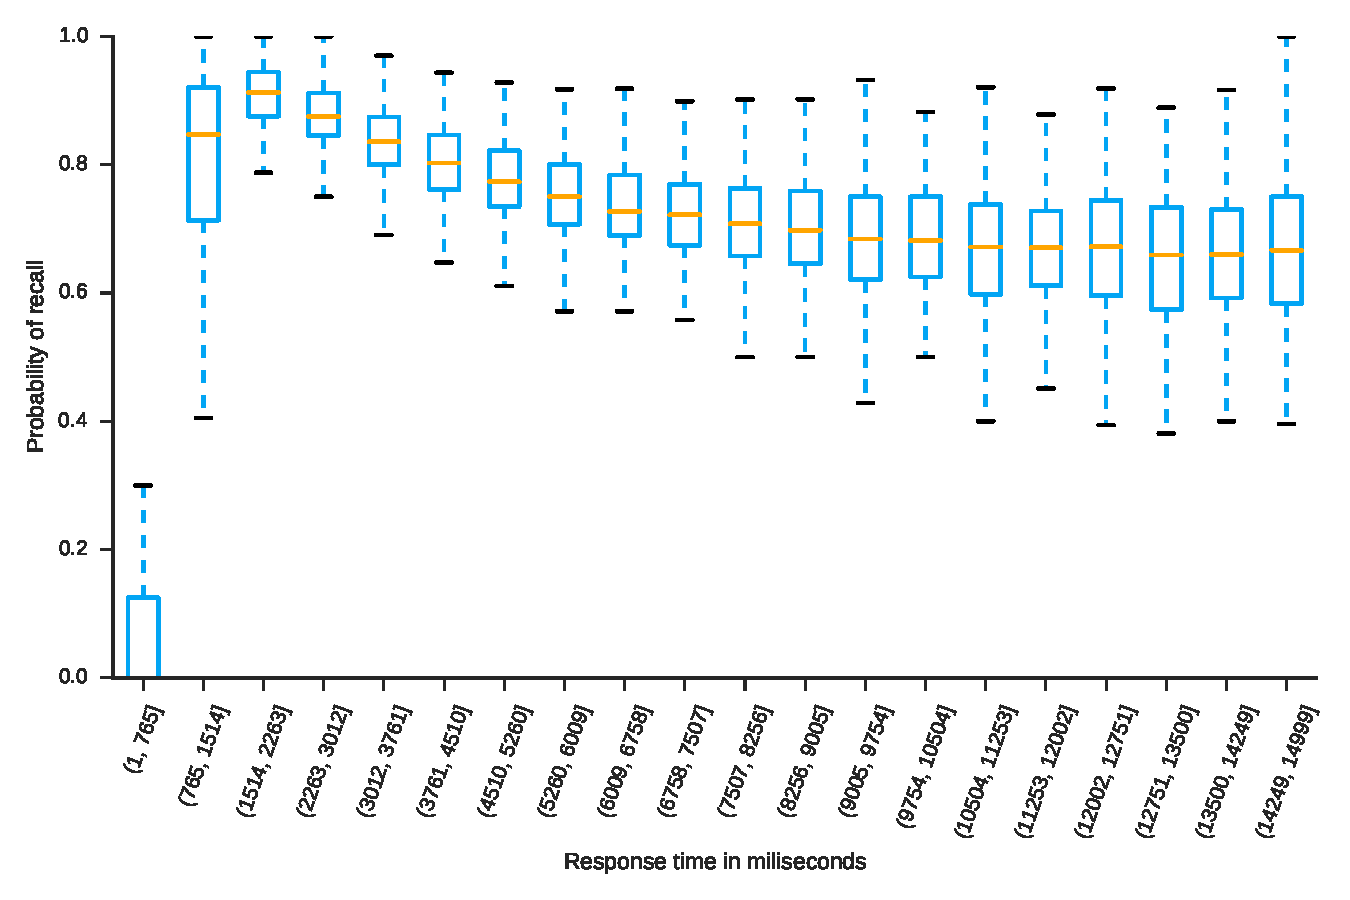
\includegraphics[width=\textwidth]{img/response-time}
  \caption{Relation between students' response time and probability of recall. Each box represents probabilities from all countries that belong in the relevant interval of response times.}
  \label{fig-response-time}
\end{figure}

\section{Memory Decay}

In this chapter we evaluate and analyze several models with the focus on memory decay and forgetting. Since we use abbreviations for the models, here is a list of all evaluated models as they occur in our experiments:

\begin{itemize}
  \item \textbf{PFA} -- this is the original performance factor analysis which we described in chapter~\ref{pfa}. Our implementation, however doesn't consider multiple knowledge components as there is only one.
  \item \textbf{PFA/E} -- a version of the original PFA model with some aspects of Elo model we depicted in chapter~\ref{pfae}.
  \item \textbf{PFA/E/T} -- an extended version of the PFA/E model which adapts the idea of a time effect function. We presented the model in chapter~\ref{pfaet}. In our analysis we examined several time effect functions.
  \item \textbf{PFA/G} -- another version of the original PFA model with a decay factor, the characteristics of the model were outlined in chapter~\ref{pfag}. The implementation doesn't consider multiple knowledge components.
  \item \textbf{PFA/G/T} -- our version of the PFA/G model which uses a time effect function instead of a decay factor. The differences we stated in chapter~\ref{pfagt}.
\end{itemize}

Note that in some analyses we also use the Elo model briefly described in chapter~\ref{elo} for the estimation of prior knowledge.

\subsection{Parameters}

Standard PFA model has 3 parameters, the initial difficulty of an item $\beta$, weight of each success $\gamma$ and failure $\delta$. In cases where we use Elo model for prior knowledge estimation, we can replace the parameter $\beta$ with $\theta_s - b_c$ which leaves us with only 2 parameters we need to estimate. Nevertheless, a time effect function has to be chosen as well for the PFA/E/T and PFA/G/T models.

\subsection*{Time Effect Functions}

In chapter~\ref{memory} we mentioned that forgetting usually respects the power law, which is often true in cases where the students have no prior knowledge of the practiced material. We tested several simple analytical function:

\begin{itemize}
  \item $f(t) = a - b \cdot \log(t)$
  \item $f(t) = a e^{b t}$
  \item $f(t) = a / t$
\end{itemize}

Each of these time effect functions can be seen on the figure~(TODO: figure) with logarithmically scaled $x$-axis. 

\subsection*{Calibration}

\subsection{Evaluation}
